\section{Controlled Evaluation}
Generative agents, both as individual agents and as groups, aim to produce believable behavior based on their environment and experiences. In our evaluation, we investigate the capacity and limitations of generative agents. Do individual agents properly retrieve past experiences and generate believable plans, reactions, and thoughts that shape their behavior? Does a community of agents demonstrate information diffusion, relationship formation, and agent coordination across different pockets of the community?

We evaluate generative agents in two stages. We begin with a more tightly controlled evaluation in this section, where we individually assess agent responses to understand whether they generate believable behavior in narrowly defined contexts. Then, in our end-to-end analysis of the agent community over two full game days, we investigate their emergent behavior as a collective, as well as errors and boundary conditions.

\subsection{Evaluation Procedure}
To assess generative agents in Smallville, we take advantage of the fact that generative agents will respond to natural language questions. So, we ``interview'' agents to probe their ability to remember past experiences, plan future actions based on their experiences, react appropriately to unexpected events, and reflect on their performance to improve their future actions. To respond to these questions properly, the agents must successfully retrieve and synthesize information. Our dependent variable is the \textit{believability} of the behavior, a central dependent variable in prior work on agents (e.g.,~\cite{22_bates1994role}). 

The interview includes five question categories, each designed to assess one of the five key areas: maintaining self-knowledge, retrieving memory, generating plans, reacting, and reflecting. For each category, we ask five questions that challenge the agents to demonstrate their abilities in that specific area:
\begin{itemize}
\item Self-knowledge: We ask questions such as “Give an introduction of yourself” or “Describe your typical weekday schedule in broad strokes” that require the agent to maintain an understanding of their core characteristics.
\item Memory: We ask questions that prompt the agent to retrieve particular events or dialogues from their memory to answer properly, such as “Who is [name]?” or “Who is running for mayor?”
\item Plans: We ask questions that require the agent to retrieve their long-term plans, such as “What will you be doing at 10 am tomorrow?” 
\item Reactions: As a baseline of believable behavior, we present hypothetical situations for which the agent needs to respond believably: “Your breakfast is burning! What would you do?”
\item Reflections: We ask questions that require the agents to leverage their deeper understanding of others and themselves gained through higher-level inferences, such as “If you were to spend time with one person you met recently, who would it be and why?”
\end{itemize}
The full list of questions and a sample of agent responses are included in Appendix \ref{sec:interview-questions}.

Agents were sampled from the end of a two game day simulation with the full architecture, during which they had accumulated a number of interactions and memories that would shape their responses. To gather feedback on the believability of the responses, we recruited participants as human evaluators and tasked them with watching a replay of a randomly chosen agent's life in Smallville. Participants had access to all information stored in the agent's memory stream.

The study followed a within-subjects design, where 100 participants compared interview responses generated by four different agent architectures and a human-authored condition for the same agent. The experiment displayed one randomly chosen question from each of the five question categories, along with the agent's responses generated from all conditions. The evaluators ranked the believability of the conditions from most to least believable.

\subsection{Conditions}
All conditions were used to independently answer each of the interview questions. We compared the generative agent architecture to ablations that disabled the agents' access to some or all of its three types of memory in its memory stream---observation, reflection, and planning---and to a \crdraft{human crowdworker-authored condition}. There are three ablated architectures: a \textit{no observation, no reflection, no planning} architecture without access to anything in the memory stream such as observations, plans, and reflections; a \textit{no reflection, no planning} architecture with access to observations in the memory stream but no access to plans or reflections; and a \textit{no reflections} architecture with access to observations and plans but without access to reflections. The \textit{no observation, no reflection, no planning} condition effectively represents the previous state of the art for agents created through large language models~\cite{9_park2022socialsimulacra,binz2023using,63_horton2023large}. Architectures were given equivalent access to all memories accrued by the agent up until the moment of the interview, so the differences observed here likely represent a conservative estimate of the true differences: in reality, the ablated architectures would not have followed the same path as the full architecture through the two-day simulation. We chose to design the experiment this way as re-simulating for each architecture would cause the simulations to diverge into different states, making comparison challenging.

In addition to the ablation conditions, \crdraft{we added a condition with human crowdworker-authored behavior intended to provide a human baseline. We do not intend this baseline to capture maximal human expert performance; instead, we aim to use this condition to identify whether the architecture meets a basic level of behavioral competency.} This ensures that we are not solely comparing ablations to each other without a behavioral grounding. We recruited a unique \crdraft{worker} for each of the 25 agents and tasked them with watching a replay of that agent's sandbox life and inspecting its memory stream. We then asked the \crdraft{workers} to roleplay and author responses to the interview questions in the voice of the agent whose replay they watched. To ensure that the \crdraft{crowdworker-authored responses} met at least a baseline expectation of quality, the first author manually inspected the \crdraft{workers'} responses to the question "Describe your typical weekday schedule in broad strokes" to confirm that the responses were in coherent sentences and in the voice of the agent. Four sets of \crdraft{crowdworker-authored responses} did not meet these criteria and were re-generated by other workers.

\subsection{Human Evaluators}
We required that our evaluators be in the U.S., fluent in English, and older than 18 years old. They were paid at a rate of \$15.00 per hour~\cite{16_rolf2015fight}, and provided consent by agreeing to a consent form approved by our institution’s IRB. We recruited 100 evaluators from Prolific, an online platform for recruiting study participants~\cite{17_prolific2022}, whose participation lasted around 30 minutes. The median age score of our participants was 4 (3=``18-24 years old'', 4=``25-34 years old''). 25 of them identified as female, 73 as male, and 2 as non-binary. 42 participants held a bachelor's degree, 5 had a higher degree, 13 had an associate's degree, and the rest had a high school diploma or some high school-level education. 73.0\% of our participants identified as Caucasian, 7.0\% as Hispanic, 6.0\% as Asian, 10.0\% as African American, and 4.0\% as other. 

\subsection{Analysis}
Our experiment produced 100 sets of rank data, where each participant ranked the five conditions by believability. To translate this rank data into interval data for interpretable comparison, we used the ranks to calculate a TrueSkill rating~\cite{79_TrueSkill} for each condition. TrueSkill is a generalization of the Elo chess rating system~\cite{80_Elo} for a multiplayer environment, and has been used by Xbox Live for player ranking based on competitive game performance. Given a set of ranked outcomes, TrueSkill outputs a mean rating value $\mu$ and standard deviation $\sigma$ for each condition. Conditions with the same rating should roughly be a toss-up, with each winning half of the comparisons between the two conditions. Higher scores indicate conditions that beat lower-ranked conditions in the rankings. 

Separately, to investigate the statistical significance of these results, we applied the Kruskal-Wallis test~\cite{Kruskal1952}, a non-parametric alternative to the one-way ANOVA, to the raw rank data. We then performed the Dunn post-hoc test~\cite{Upton2006} to identify any pairwise differences between the conditions. Finally, we adjusted the p-values for multiple comparisons in the Dunn test using the Holm-Bonferroni method~\cite{Holm1979}.

Furthermore, the first author conducted an inductive analysis~\cite{18_thomas2006general} to study the qualitative distinctions between the responses produced in each condition. We employed qualitative open coding~\cite{78_open_coding} in two phases. In the first phase, we generated codes that closely represented the generated responses at the sentence level. In the second phase, we synthesized the resulting codes from the first phase to extract higher-level themes. We utilized these themes to compare the types of responses generated in our study.

\begin{figure}[tb]
  \centering
  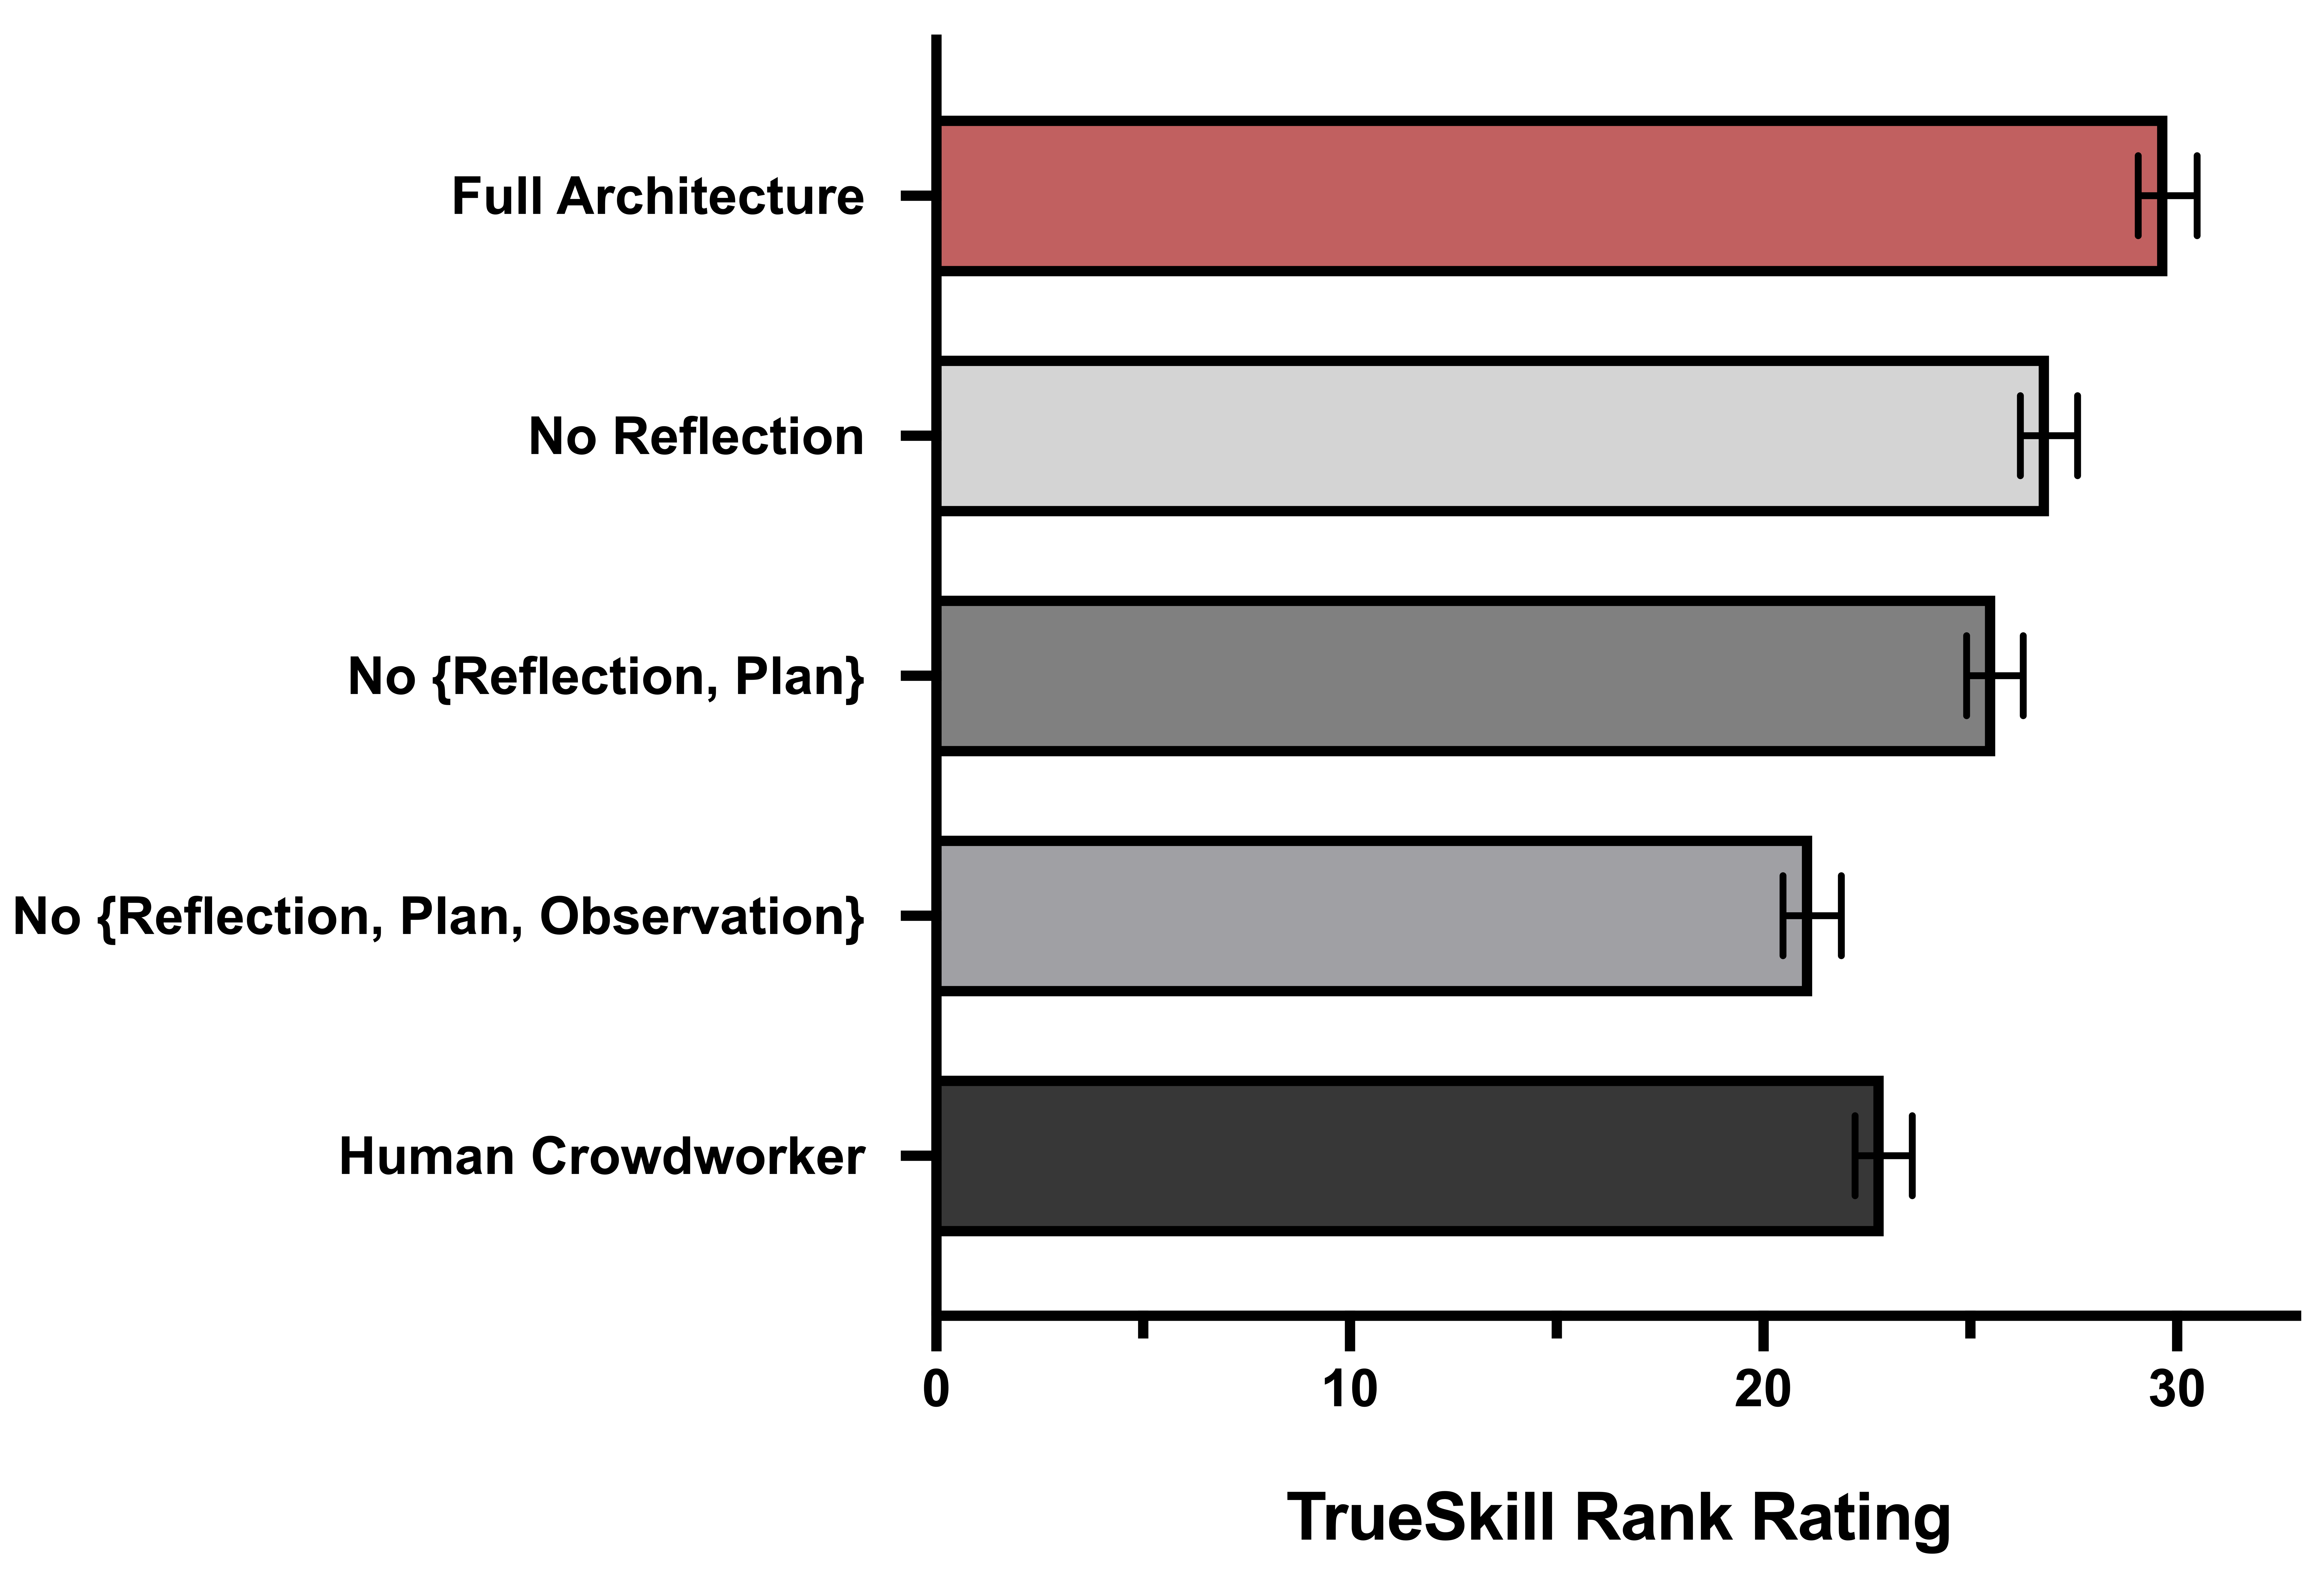
\includegraphics[width=0.97\columnwidth]{figures/figure_rank_score_comparison4.png}
  \caption{The full generative agent architecture produces more believable behavior than the ablated architectures and \crdraft{the human crowdworkers}. Each additional ablation reduces the performance of the architecture.}
  \Description{A bar graph of TrueSkill mu scores. The full architecture outperforms other conditions.}
  \label{fig:trueskill}
\end{figure}


\subsection{Results}
Our findings suggest that the full architecture of generative agents generates the most believable behavior among all the conditions. We contrast the responses of the full architecture with those of other conditions below. However, we also report that the full architecture was not without flaws and illustrate its modes of failures.

\subsubsection{The Full Architecture Bests Other Conditions} 
As seen in Figure~\ref{fig:trueskill}, the full generative agent architecture produced the most believable behavior ($\mu=29.89$; $\sigma=0.72$). Performance degraded with the removal of each component in the ablation conditions: the ablated architecture with no access to reflection was the next best ($\mu=26.88$; $\sigma=0.69$), followed by no access to reflection or planning ($\mu=25.64$; $\sigma=0.68$), and then \crdraft{the crowdworker condition} ($\mu=22.95$; $\sigma=0.69$). The ablated architecture with no access to memory, planning, or reflection performed the worst among all conditions ($\mu=21.21$; $\sigma=0.70$). TrueSkill models each condition's skill value as $\mathcal{N}(\mu,\,\sigma^{2})$, allowing us to get a sense of effect size through Cohen's d. Comparing the condition representing prior work (with no memory, planning, or reflection~\cite{9_park2022socialsimulacra,binz2023using,63_horton2023large}) to the full architecture produces a standardized effect size of $d=8.16$, or \textit{eight standard deviations}. 

A Kruskal-Wallis test confirms the overall statistical significance of the differences in ranks between the conditions ($H(4)=150.29$, $p<0.001$). Dunn post-hoc tests confirm that all pairwise differences between conditions were significant ($p<0.001$), except for the crowdworker condition and the fully ablated baseline---the two worst-performing conditions.

\subsubsection{Generative Agents Remember, but With Embellishments}
Generative agents equipped with a complete memory module are capable of recalling past experiences and answering questions in a manner that is consistent with their self-knowledge across a wide range of contexts. For instance, Abigail Chen, an animator, responded to the question, ``Give an introduction of yourself'', in a consistent and believable manner, stating her age, interests, and passion for creative projects: \gentxt{``Hi, I'm Abigail. I'm 25 years old and passionate about creative projects. I like to work on art and animation projects, and I'm always looking for new ways to combine art and technology.''} Without access to her observational memory, Abigail denied awareness of Rajiv Patel, an acquaintance in the sandbox world. But with the aid of memory, she could successfully recall Rajiv and describe him: \gentxt{``Rajiv Patel is an incredible person. He is very enthusiastic about projects that involve poetry, artwork.''}

Generative agents' memory was not without flaws: they can fail to retrieve the correct instances from their memory. For instance, when asked about the local election, Rajiv Patel responded with \gentxt{``I haven't been following the election too closely,''} even though he had heard about Sam's candidacy. In some cases, the agents would retrieve an incomplete memory fragment: when Tom was asked about Isabella's Valentine's Day party, he responded \gentxt{``Uh, I’m actually not sure if there is a Valentine’s Day party. But I do remember that I need to discuss the upcoming local mayoral election and my thoughts on Sam Moore with Isabella Rodriguez at the party, if one is happening!''} In this case, Tom retrieved the memory where he and Isabella planned to discuss the election at the party, but not the memory where he heard about the party, leading Tom to be certain of what he's supposed to do at the party but uncertain if the party actually exists in the first place.

At times, the agents hallucinated embellishments to their knowledge. It was rare for the agents to completely fabricate their knowledge: they may fail to recall certain events having taken place and respond by acknowledging their lack of memory. However, they did not affirmatively claim to have experienced something they had not. Nonetheless, they still exhibited instances of hallucination where they embellished their knowledge. For example, Isabella was aware of Sam's candidacy in the local election, and she confirmed this when asked. However, she also added that \gentxt{``he's going to make an announcement tomorrow''}, even though Sam and Isabella had not discussed any such plans. Agents may also embellish their knowledge based on the world knowledge encoded in the language model used to generate their responses. This was observed when Yuriko described her neighbor, Adam Smith, as an economist who \gentxt{``authored Wealth of Nations''}, a book written by an 18th-century economist of the same name.

\subsubsection{Reflection Is Required for Synthesis}
Reflection was an advantage for generative agents when making decisions that required a deeper synthesis of their experiences. For instance, when asked what she might get Wolfgang Schulz for his birthday, Maria Lopez, with no access to reflection, responded by acknowledging her uncertainty, stating that she did not know what Wolfgang likes, despite having had many interactions with him. However, with access to reflection memories, Maria answered confidently, \gentxt{``Since he's interested in mathematical music composition, I could get him something related to that. Maybe some books about music composition or something related, or maybe some special software he could use for that.''} 

